%______________________________________________________________________________________________________________________
% @brief    LaTeX2e Resume for Kamil K Wojcicki
\documentclass[line,a4paper]{resume}

% Allow text with accents and Umlauts.
\usepackage[ansinew]{inputenc}
%\usepackage{pifont}
\usepackage[english,austrian]{babel}
%\usepackage[T1]{fontenc}
\usepackage{graphicx,wrapfig,multirow}
\usepackage{url}
\usepackage{amsmath}
\usepackage[colorlinks=true, a4paper=true, pdfstartview=FitV, linkcolor=blue, citecolor=blue, urlcolor=blue]{hyperref}
% \pdfcompresslevel=9

\newcommand{\superscript}[1]{\ensuremath{^{\text{#1}}}}
\newcommand{\subscript}[1]{\ensuremath{_{\text{#1}}}}
%\renewcommand{\familydefault}{\sfdefault}

\usepackage{ifthen}
\newboolean{WithPhoto}

% Set to true for Austria Contact, false for NJ
\setboolean{WithPhoto}{true} 

% Headers and footers
\usepackage{fancyhdr}

%______________________________________________________________________________________________________________________
\begin{document}

 \fontencoding{T1}
  \fontfamily{phv}
  \fontseries{m}
  \fontshape{n}
  \fontsize{10}{12}
  \selectfont


\name{\Large Matthew D. DiFranco, PhD \hspace{33mm} {\small mdifranc@gmail.com/+43(0)660 142 7331}}
\pagestyle{fancy}	
\lhead{}
\chead{}
\rhead{\leftmark}
\lfoot{}
\cfoot{}
\rfoot{\thepage}

\renewcommand{\headrulewidth}{0pt}
\renewcommand{\footrulewidth}{0.4pt}
\fancyhfoffset[L]{\hoffset}

% Defines the height of the header.
\setlength{\headheight}{10pt}
\setlength{\textheight}{725pt}

% BEGIN COVER LETTER
% {
% \fontfamily{sffamily}\selectfont
% \normalsize \vspace{14mm}
% Matthew D. DiFranco, PhD  \vspace{-4mm}
% 
% Nedergasse 8/5 \vspace{-4mm}
% 
% 1190 Wien \vspace{-4mm}
% 
% Austria
% 
% 7. October 2015
% 
% Medizinische Universit{\"a}t Wien  \vspace{-4mm}
% 
% Personalabteilung \vspace{-4mm}
% 
% Spitalgasse 23 \vspace{-4mm}
% 
% A-1090 Wien \vspace{-4mm}
% 
% Austria \vspace{4mm}
% % 
% \large
% 
% \textbf{Betreff: Antrag f{\"u}r eine Qualifizierungsvereinbarung (QV)} \vspace{4mm}
% 
%Sehr geehrte Damen und Herren, \vspace{4mm}
% 
%ich schicke Ihnen mit dieser Sendung meinen Antrag f{\"u}r einen Qualifizierungsvereinbarung im Zentrum f{\"u}r medizinische Physik und biomedizinische Technik. Im Anhang finden Sie eine aktuelle CV inklusive eine Liste von Lehrt{\"a}tigkeiten, eine Publikationsliste samt Aufzeichnung der f{\"u}nf Beste, und eine ausgef{\"u}llte Fact Sheet und Formular zum ausw{\"a}rtigen Forschungs-/Lehraufenthalt.
% 
%Bez{\"u}glich eines ausw{\"a}rtigen Aufenthaltes habe ich mehrere Jahren Erfahrung als Univerist{\"a}tsassistent in London, UK und Innsbruck, und auch als Doktorand in Dublin, Irland. W{\"a}hrend der Zeit als Universit{\"a}tsassistent und Doktorand habe ich auch Lehrt{\"a}tigkeiten durchgef{\"u}hrt.
%
%Bei Nachfragen zu meinen Angaben stehe ich Ihnen gerne zu Verf{\"u}gung.
% 
% Mit freundlichen Gr{\"u}{\ss}en, \vspace{4mm}
% 
% Matthew D. DiFranco, PhD \vspace{-4mm}
%  }

% END COVER LETTER
\newpage
\begin{resume}

    %__________________________________________________________________________________________________________________
    % Contact Information
\section{\mysidestyle}\vspace{2mm}
	
\ifthenelse {\boolean{WithPhoto}}
{
\begin{table}[h]
 \begin{tabular}{@{}p{40mm}@{}p{60mm}@{}p{70mm}}
  \multirow{10}{*}{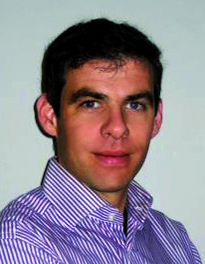
\includegraphics[height=45mm]{IMG_8089_35x45mm.jpg}}
  % & \multicolumn{2}{l}{\hspace{-2mm}\textbf{Born:} October 13, 1977, New Jersey, USA} \\
  & \textbf{Home Address} & \textbf{Work Address} \\
  & Nedergassee 8/5 & Medical University of Vienna \\
  & 1190 Vienna, Austria & Center for Medical Physics and Biomedical Engineering\\
  & & Waehringer Guertel 18-20 \\
  & & 1090 Vienna, Austria \\[3mm]
  & phone: +43 (0) 660 142 7331 & +43 (0) 1 40400 19880 \\
  & mdifranc@gmail.com & matthew.difranco@meduniwien.ac.at \\[5mm]
  % & \multicolumn{2}{l}{\hspace{-2mm}\textbf{Citizenship:} United States of America} \\
  & \multicolumn{2}{l}{\hspace{-2mm}\textbf{Languages:} English, German} \\[5mm]
\multicolumn{3}{@{}p{\textwidth}}{\noindent\textbf{Research Interests:} medical image computing, multi-parametric imaging analysis, computer aided detection and diagnosis, machine learning, image guided surgery, statistical shape modeling, microscopic imaging} \\ [5mm]
 \end{tabular}
\end{table}
}
{
\begin{table}[h]
 \begin{tabular}{@{}p{85mm}@{}p{85mm}}
  \textbf{Home Address} & \textbf{Work Address} \\[2mm]
  Nedergassee 8/5 & Medical University of Vienna \\
  1190 Vienna, Austria & Center for Medical Physics and Biomedical Engineering\\
  & Waehringer Guertel 18-20 \\
  & 1090 Vienna, Austria \\[3mm]
  phone: +43 (0) 660 142 7331 & +43 (0) 1 40400 19880 \\
  mdifranc@gmail.com & matthew.difranco@meduniwien.ac.at \\[5mm]
 %  \multicolumn{2}{l}{\hspace{-2mm}\textbf{Citizenship:} United States of America} \\
  \multicolumn{2}{l}{\hspace{-2mm}\textbf{Languages:} English, German} \\[5mm]
  \multicolumn{2}{@{}p{\textwidth}}{\noindent\textbf{Research Interests:} medical image computing, multi-parametric imaging analysis, computer aided detection and diagnosis, machine learning, image guided surgery, statistical shape modeling, microscopic imaging} \\ [5mm]
 \end{tabular}
\end{table}
}

%__________________________________________________________________________________________________________________
    % Research Interests
    % \section{\mysidestyle Research Interests}\vspace{3mm}
    % 
    % Medical image analysis, computer aided detection and diagnosis, computer vision, pattern recognition machine learning, color and texture analysis, and image retrieval
 
 %__________________________________________________________________________________________________________________
    % Education
    \section{\mysidestyle Education}\vspace{3mm}
    \textbf{University College Dublin:}  Doctor of Philosophy, Computer Science \hfill Oct. 2006 -- Aug. 2010 \vspace{2mm}\\%
     \textbf{University College London:}  Master of Research, Computer Science \hfill Sep. 2003 -- Sep. 2004 \vspace{2mm}\\%
     \textbf{Drexel University, Philadelphia:}  Bachelor of Science (Hon.), Materials Engineering \hfill Sep. 1995 -- Jun. 2000 \vspace{2mm}\\%
     \textbf{Christian Brothers Academy, Lincroft, NJ:}  High School Diploma \hfill Sep. 1991 -- Jun. 1995 \vspace{1mm}\\%     
%__________________________________________________________________________________________________________________
 	% Research Experience
	\section{\mysidestyle Research Experience}\vspace{3mm}
	% Research 1
	\begin{minipage}{\textwidth}
	\textbf{Medical University of Vienna:} Imaging Scientist (Post-doc) \hfill May 2014 -- present \\%
	\textsl{Center for Medical Physics and Biomedical Engineering}\vspace{1mm}\\
	 Integration of digital pathology analysis with in-vivo hybrid imaging (PET/MR) to develop models of tumor heterogeneity and therapy response.\vspace{1mm}\\%
	\end{minipage}
	% Research 2
	\begin{minipage}{\textwidth}
	\textbf{Medical University of Vienna:} Marie Curie Post-doctoral Fellow \hfill May 2012 -- May 2014 \\%
	\textsl{Computational Imaging Research Lab}\vspace{1mm}\\
	  \textbf{BoneMATCH Project:} Multimodal, multi-scale bone image analysis to improve recognition and detection of microarchitectural features and changes in cortical and trabecular bone.\\vspace{1mm}\\%
	\end{minipage}
	% Research 3
	\begin{minipage}{\textwidth}
	\textbf{Medical University of Innsbruck:} Post-doc Research Assistant \hfill Oct 2010 -- May 2012 \\%
	\textsl{4D Visualization Lab, University Clinic for ENT Medicine}\vspace{1mm}\\
	  \textbf{Rhinospider Project:} Development of an implantable device designed to improved navigation accuracy in neurosurgery as well as surgical interventions in the lateral and frontal skull base. \vspace{1mm}\\%
	\end{minipage}
	% Research 4
	\begin{minipage}{\textwidth}
	\textbf{University College Dublin:} Doctoral Candidate \hfill Oct. 2006 -- Aug. 2010 \\%
	\textsl{Machine Learning Group, School of Computer Science and Informatics}\vspace{1mm}\\
	  \textbf{PhD Thesis:} Automated cancer detection in whole-mount prostate histopathology images.\vspace{1mm}\\%
	\end{minipage}
	% % Research 5
	\begin{minipage}{\textwidth}
	\textbf{University College London:} Research Assistant \hfill Jun. 2005 -- Sep 2006 \\%
	\textsl{Biomedical Informatics Unit, Eastman Dental Institute}\vspace{1mm}\\
	  Statistical shape modeling of face and palate for shape anomaly detection in genetic syndromes (US National Institutes of Health grant number 5P50DE016215-05). \vspace{1mm}\\%
	\end{minipage}
	% % Research 6
	\begin{minipage}{\textwidth}
	\textbf{University College London:} Graduate Student \hfill Sep. 2003 -- Sep 2004 \\%
	\textsl{Department of Computer Science}\vspace{1mm}\\
	\textbf{Masters Thesis:} Meshless finite element methods for modeling diffuse light propagation in tissue. \vspace{1mm}\\%
	\end{minipage}
		% % Research 7
	\begin{minipage}{\textwidth}
	\textbf{Drexel University} Undergraduate Student \hfill Sep. 1999 -- Jun 2000 \\%
	\textsl{Department of Materials Engineering}\vspace{1mm}\\
	\textbf{Bachelors Thesis:} Characterization of thermal spray of titanium silicocarbide (Ti\subscript{3}SiC\subscript{2}) powders.  \vspace{1mm}\\%
	\end{minipage}
%__________________________________________________________________________________________________________________
    % Professional Experience
    \section{\mysidestyle Professional Experience}\vspace{3mm}
	\begin{minipage}{\textwidth}
	\textbf{Smart \& Associates, Philadelphia, Pennsylvania} \textsl{Senior Consultant} \hfill Sep. 2002 -- Aug 2003 \\%
	Business development experience, including proposal to large pharmaceutical company for outsourcing of Tier 3 support organization responsible for maintenance, development, and troubleshooting of a 5000 seat Siebel ePharma implementation. Developed and implemented data analysis tools for process quality review of a Tier 3 Siebel ePharma support organization, tax record assessment, and document management. \vspace{1mm}\\%
	\end{minipage}
	\begin{minipage}{\textwidth}
	\textbf{Accenture, Philadelphia, Pennsylvania} \textsl{Technology Analyst}  \hfill Sep. 2000 -- Aug. 2002 \\
    	Extensive software development experience, including lead developer on broadband ordering and provisioning tool project for large telecommunications client. Supported customer relationship management (CRM) software strategy assessment for large telecommunications company, including interface with software vendors on behalf of client and organization of two-day client workshop for 30 stakeholders. Planned and conducted client training sessions, and performed client engagement quality analysis. \vspace{1mm} \\
	\end{minipage}
	\begin{minipage}{\textwidth}
		\textbf{LaFrance Corporation, Concordville, Pennsylvania} \textsl{Associate Design Engineer} \hfill Mar. 1999 -- Sep. 1999 \\
    	Initiated and developed new product concepts specific to customer needs utilizing AutoCAD and Pro/Engineer 3D computer-aided design software. Acquired knowledge in tooling of molds and operation of injection molder. \vspace{1mm} \\
	\end{minipage}
	\begin{minipage}{\textwidth}
	    \textbf{W.L. Gore and Associates, Elkton, Maryland} \textsl{Materials Development Associate} \hfill Mar. 1999 -- Sep. 1999 \\
		\textbf{Project:} Hard-drive adsorbent breather filter performance and processing optimization \vspace{1mm}\\%
	\end{minipage}
	\begin{minipage}{\textwidth}
		   \textbf{McNeil Consumer Products, Fort Washington, Pennsylvania} \textsl{Research Assistant} \hfill Mar. 1997 -- Sep. 1997 \\
		\textbf{Project: }Formulation and process development of novel children's drug delivery system.\\%
	\end{minipage}

%__________________________________________________________________________________________________________________
	% % Teaching Experience
	\section{\mysidestyle Teaching Experience}\vspace{1mm}
    \textbf{Medical University of Vienna, Austria} \hfill May 2013 - present \\
    \textsl{Bachelor's and master's project supervision: Dominik Hofer (TU Wien)} \\
    \textsl{Master's supervision: Michaela Weingant (TU Wien)} \vspace{1mm}\\%
    \textbf{University College Dublin, Ireland} \hfill Jan. 2007 -- May 2010\\
    \textsl{Senior Postgraduate Demonstrator, School of Computer Science and Informatics} \\
     Machine Learning, Discrete Mathematics, Algorithmic Problem Solving, Software Engineering, Intro. to Artificial Intelligence, Intro. to Computer Architecture, Intro. to C Programming \vspace{1mm}\\%
    \textbf{Queen Mary College London} \hfill January 2004 -- June 2006\\
    \textsl{Teaching Assistant, Open and Distance Learning Unit} \vspace{1mm}\\%
    \textbf{Drexel University, Philadelphia, Pennsylvania} \hfill September 1999 -- June 2000\\
    \textsl{Writing Tutor, Drexel University Writing Program}

%__________________________________________________________________________________________________________________
    % Computer Skills
    \section{\mysidestyle Computing Experience}\vspace{2mm}

    \textbf{Image Processing and Scientific Computing} Matlab, ITK, VTK, IGSTK, ImageJ, R, Python, OMERO \\
    \textbf{Application Development} Java, C++, Qt \\
    \textbf{Mechanical Drawing and Design} AutoCAD, AutoDesk Inventor \\
    \textbf{Web development} PHP/MySQL, HTML \\
    \textbf{Database Development} Access, Oracle, SQL Server, PostgreSQL \\
    % \textbf{Miscellaneous} \LaTeXe, MS Office
	
%__________________________________________________________________________________________________________________
% % Conferences

\section{\mysidestyle Conferences and Seminars}\vspace{2mm}
% Conf 1
\noindent
\begin{minipage}[t]{0.20\linewidth}
\textbf{Oct. 5, 2015}
\end{minipage}
\begin{minipage}[t]{0.80\linewidth}\raggedright
Poster Presentation: \emph{Ensemble Prostate Tumor Classification in H\&E Whole Slide Imaging via Stain Normalization and Cell Density Estimation} \\*
MICCAI Workshop on Machine Learning in Medical Imaging, Munich, Germany
\end{minipage}

% Conf 1
\noindent
\begin{minipage}[t]{0.20\linewidth}
\textbf{Sept. 21-22, 2015}
\end{minipage}
\begin{minipage}[t]{0.80\linewidth}\raggedright
Session Chair and Invited Talk: \emph{Whole-slide Imaging Informatics in Clinical Imaging Studies}\\*
Digital Pathology Congress Asia, Kuala Lumpur, Malaysia
\end{minipage}

% Conf 1
\noindent
\begin{minipage}[t]{0.20\linewidth}
\textbf{Feb. 21-26, 2015}
\end{minipage}
\begin{minipage}[t]{0.80\linewidth}\raggedright
Poster Presentation: \emph{Performance assessment of automated tissue characterization for prostate H and E stained histopathology}\\*
2015 SPIE Medical Imaging, Orlando, Florida, USA
\end{minipage}

% Conf 2
\noindent
\begin{minipage}[t]{0.20\linewidth}
\textbf{Sept. 12-15, 2014}
\end{minipage}
\begin{minipage}[t]{0.80\linewidth}\raggedright
Invited Talk: \emph{Bone and Muscle Working Group: Novel Approaches to Assessment of Microarchitectural Bone Changes}\\*
Poster Presentation: \emph{Atlas-based Correlation of local Trabecular Directionality and Deformation with Serum Markers of Bone Turnover in Lung Transplant Recipients in a Longitudinal Setting}\\*
2014 American Society of Bone Mineral Research (ASBMR) Annual Meeting, Houston, Texas, USA
\end{minipage}

% Conf 3
\noindent
\begin{minipage}[t]{0.20\linewidth}
\textbf{Mar. 6-10, 2014}
\end{minipage}
\begin{minipage}[t]{0.80\linewidth}\raggedright
Oral Presenter: \emph{Denoising of HRpQCT scans via dicitionary learning for improved spatio-temporal morphometry analysis}\\*
Oral Co-author: \emph{Effects of recent lung transplantation on cortical and trabecular microarchitecture and bone strength in men and women}\\*
20\superscript{th} European Congress of Radiology (ECR) 2014, Vienna, Austria
\end{minipage}

% Conf 3
\noindent
\begin{minipage}[t]{0.20\linewidth}
\textbf{Dec. 1-6, 2013}
\end{minipage}
\begin{minipage}[t]{0.80\linewidth}\raggedright
Oral Co-author: \emph{Impaired Cortical and Trabecular Bone Microarchitecture in Female and Male Lung Transplant Recipients}\\*
99\superscript{th} Scientific Assembly and Annual Meeting of the Radiological Society of North America (RSNA) 2013, Chicago, Illinois, USA
\end{minipage}

% Conf 3
\noindent
\begin{minipage}[t]{0.20\linewidth}
\textbf{Oct. 4-7, 2013}
\end{minipage}
\begin{minipage}[t]{0.80\linewidth}\raggedright
Poster Presentation: \emph{Sub-compartmental Bone Morphometry Analysis in Longitudinal HRpQCT Scans with Application to Chronic Kidney Disease}\\*
Poster Co-author: \emph{Severe Alterations in Cortical and Trabecular Bone Microarchitecture in Lung Transplant Recipients}\\*
2013 American Society of Bone Mineral Research (ASBMR) Annual Meeting, Baltimore, Maryland, USA
\end{minipage}

% Conf 3
\noindent
\begin{minipage}[t]{0.20\linewidth}
\textbf{May 23-24, 2013}
\end{minipage}
\begin{minipage}[t]{0.80\linewidth}\raggedright
Poster Presentation: \emph{Mineralized Bone Segmentation in HR-pQCT Images using Dictionary Learning Methods}\\*
The 37th Annual Workshop of the Austrian Association for Pattern Recognition (AAPR), Innsbruck, Austria
\end{minipage}

% Conf 3
\noindent
\begin{minipage}[t]{0.20\linewidth}
\textbf{Oct. 12-15, 2012}
\end{minipage}
\begin{minipage}[t]{0.80\linewidth}\raggedright
2012 American Society of Bone Mineral Research (ASBMR) Annual Meeting, Minneapolis, Minnesota, USA
\end{minipage}

% Conf 3
\noindent
\begin{minipage}[t]{0.20\linewidth}
\textbf{Oct. 1-5, 2012}
\end{minipage}
\begin{minipage}[t]{0.80\linewidth}\raggedright
International Conference on Medical Image Computing and Computer Assisted Intervention (MICCAI), Nice, France
\end{minipage}

% Conf 1
\noindent
\begin{minipage}[t]{0.20\linewidth}
\textbf{Jul. 4-13, 2012}
\end{minipage}
\begin{minipage}[t]{0.80\linewidth}\raggedright
Lecturer and Organizer:Summer School on Image Processing (SSIP 2012), Vienna, Austria
\end{minipage}

% Conf 1
\noindent
\begin{minipage}[t]{0.20\linewidth}
\textbf{Sep. 18, 2011}
\end{minipage}
\begin{minipage}[t]{0.80\linewidth}\raggedright
Oral Presentation: \emph{Extending the tracking device support in the Image-Guided Surgery Toolkit (IGSTK): CamBar B2, EasyTrack 500, and Active Polaris}\\*
MICCAI Workshop on Systems and Architectures for Computer Assisted Interventions, Toronto, Ontario, Canada
\end{minipage}

% Conf 2
\noindent
\begin{minipage}[t]{0.20\linewidth}
\textbf{Sep. 24, 2009}
\end{minipage}
\begin{minipage}[t]{0.80\linewidth}\raggedright
Oral Presentation: \emph{Mapping Suspected Prostatic Carcinoma Using Smoothed Co-occurrence Texture Features}\\*
MICCAI Workshop on Optical Tissue Image Analysis in Microscopy, Histopathology and Endoscopy (OPTIMHisE), London, UK
\end{minipage}

% Conf 3
\noindent
\begin{minipage}[t]{0.20\linewidth}
\textbf{Sep. 21-23, 2009}
\end{minipage}
\begin{minipage}[t]{0.80\linewidth}\raggedright
International Conference on Medical Image Computing and Computer Assisted Intervention (MICCAI), London, UK
\end{minipage}

% Conf 4
\begin{minipage}[t]{0.20\linewidth}
\textbf{Mar. 6-10, 2009}
\end{minipage}
\begin{minipage}[t]{0.80\linewidth}\raggedright
European Congress of Radiology, Vienna, Austria
\end{minipage}

% Conf 5
\noindent
\begin{minipage}[t]{0.20\linewidth}
\textbf{Dec. 18-21, 2008}
\end{minipage}
\begin{minipage}[t]{0.80\linewidth}\raggedright
Presentation: \emph{Automated Detection of Prostate Cancer in Histopathology Slides}\\*
Laboratory for Computational Imaging and Bioinformatics, Dept. of Biomedical Engineering, Rutgers University, New Jersey, USA

\end{minipage}

% Conf 6
\noindent
\begin{minipage}[t]{0.20\linewidth}
\textbf{Sep. 7-9, 2008}
\end{minipage}
\begin{minipage}[t]{0.80\linewidth}\raggedright
International Conference on Medical Image Computing and Computer Assisted Intervention (MICCAI), New York City, USA
\end{minipage}

% Conf 7
\noindent
\begin{minipage}[t]{0.20\linewidth}
\textbf{Sep. 6, 2008}
\end{minipage}
\begin{minipage}[t]{0.80\linewidth}\raggedright
Poster Presentation: \emph{Automated Gleason Scoring of Prostatic Histopathology Slides Using Multi-channel Co-occurrence Texture Features}\\*
MICCAI Workshop on Microscopic Image Analysis with Applications in Biology (MIAAB), New York City, USA
\end{minipage}

% Conf 8
\noindent
\begin{minipage}[t]{0.20\linewidth}
\textbf{Apr. 4, 2008}
\end{minipage}
\begin{minipage}[t]{0.80\linewidth}\raggedright
Presentation: \emph{Computer-aided Detection of Tissue Regions in Prostate Immunohistochemistry Slides}\\*
Centre for Medical Image Computing (CMIC), University College London, UK
\end{minipage}

% Conf 9
\noindent
\begin{minipage}[t]{0.20\linewidth}
\textbf{Dec. 17, 2007}
\end{minipage}
\begin{minipage}[t]{0.80\linewidth}\raggedright
Eurographics Ireland 2007, University College Dublin, Ireland
\end{minipage}

% Conf 10
\noindent
\begin{minipage}[t]{0.20\linewidth}
\textbf{Aug. 29-31, 2007}
\end{minipage}
\begin{minipage}[t]{0.80\linewidth}\raggedright
Irish Conference on Artificial Intelligence and Cognitive Science (AICS), Dublin Institute of Technology, Ireland
\end{minipage}

% Conf 11
\noindent
\begin{minipage}[t]{0.20\linewidth}
\textbf{Mar. 9-13, 2007}
\end{minipage}
\begin{minipage}[t]{0.80\linewidth}\raggedright
European Congress of Radiology, Vienna, Austria
\end{minipage}

% Conf 12
\noindent
\begin{minipage}[t]{0.20\linewidth}
\textbf{Nov. 27-28, 2006}
\end{minipage}
\begin{minipage}[t]{0.80\linewidth}\raggedright
International Workshop on Current Challenges in Kernel Methods, Brussels, Belgium
\end{minipage}
%__________________________________________________________________________________________________________________
% % Courses

\section{\mysidestyle Courses}\vspace{3mm}
% Courses 1
\begin{minipage}[t]{0.20\linewidth}
\textbf{Feb. 19-21, 2014}
\end{minipage}
\begin{minipage}[t]{0.80\linewidth}\raggedright
3\superscript{rd} T{\"u}bingen PET/MR Workshop, Universit{\"a}sklinikum T{\"u}bingen, Germany
\end{minipage}

% Courses 1
\begin{minipage}[t]{0.20\linewidth}
\textbf{Jul. 11-18, 2009}
\end{minipage}
\begin{minipage}[t]{0.80\linewidth}\raggedright
21\superscript{st} International School for Computer Science Researchers: Molecular and Medical Image Analysis and Bioinformatics, Lipari, Sicily, Italy
\end{minipage}

% Courses 2
\noindent
\begin{minipage}[t]{0.20\linewidth}
\textbf{2008 - 2009}
\end{minipage}
\begin{minipage}[t]{0.80\linewidth}\raggedright
Goethe-Institut Dublin, German Levels A1.2, A2.1, and A2.2
\end{minipage}

% Courses 2
\noindent
\begin{minipage}[t]{0.20\linewidth}
\textbf{Sep. 10, 2008}
\end{minipage}
\begin{minipage}[t]{0.80\linewidth}\raggedright
Designing Multi-scale Medical Image Analysis Algorithms, MICCAI 2008 Tutorial, New York City, USA
\end{minipage}

% Courses 3
\noindent
\begin{minipage}[t]{0.20\linewidth}
\textbf{Jul. 7-16, 2008}
\end{minipage}
\begin{minipage}[t]{0.80\linewidth}\raggedright
16\superscript{th} Summer School on Image Processing, Technical University of Vienna, Austria\\*
Team project second prize \emph{Landmark Recognition in Photographs}
\end{minipage}

% Courses 4
\noindent
\begin{minipage}[t]{0.20\linewidth}
\textbf{Feb. 9-15, 2008}
\end{minipage}
\begin{minipage}[t]{0.80\linewidth}\raggedright
High Content Screening Technologies Course, Institute of Molecular Medicine, Trinity College Dublin, Ireland
\end{minipage}
  %__________________________________________________________________________________________________________________
%     % Other Stuff
    \section{\mysidestyle Other Interests}\vspace{2mm}

		\noindent
		\begin{minipage}[t]{0.25\linewidth}
		\textbf{April. 2014 - present}
		\end{minipage}
		\begin{minipage}[t]{0.75\linewidth}\raggedright
		\textbf{VE Brewers Slow-pitch Softball, Spenadlwiese, Vienna, Austria}
		\end{minipage}

		\noindent
		\begin{minipage}[t]{0.25\linewidth}
		\textbf{Jan. 2013 - May 2014}
		\end{minipage}
		\begin{minipage}[t]{0.75\linewidth}\raggedright
		\textbf{Basket Flames Basketball Sportverein, Vienna, Austria}
		\end{minipage}

		% \noindent
		% \begin{minipage}[t]{0.25\linewidth}
		% \textbf{Mar. 2011 - Apr. 2012}
		% \end{minipage}
		% \begin{minipage}[t]{0.75\linewidth}\raggedright
		% \textbf{Flying Circus e.V. Ultimate Frisbee Team, Innsbruck, Austria}
		% \end{minipage}

		\noindent
		\begin{minipage}[t]{0.25\linewidth}
		\textbf{Sep. 2008 - Sep. 2009}
		\end{minipage}
		\begin{minipage}[t]{0.75\linewidth}\raggedright
		\textbf{Irish Flying Disc Association Development Officer}
		\end{minipage}
		
		\noindent
		\begin{minipage}[t]{0.25\linewidth}
		\textbf{Sep. 2006 - Sep. 2009}
		\end{minipage}
		\begin{minipage}[t]{0.75\linewidth}\raggedright
		\textbf{UCD Ultimate Frisbee Club, Dublin (Club Captain 2007-2008)}
		\end{minipage}

		\noindent
		\begin{minipage}[t]{0.25\linewidth}
		\textbf{Sep. 2003 - Sep. 2006}
		\end{minipage}
		\begin{minipage}[t]{0.75\linewidth}\raggedright
		\textbf{UCL Ultimate Frisbee Club, London (Mixed Captain 2006)}
		\end{minipage}
			
		\noindent
		\begin{minipage}[t]{0.25\linewidth}
		\textbf{Sep. 1997 - Jun. 2000}
		\end{minipage}
		\begin{minipage}[t]{0.75\linewidth}\raggedright
		\textbf{The Triangle, Student Newspaper at Drexel University (Editorial Board 1999-2000)}
		\end{minipage}

    %__________________________________________________________________________________________________________________
    % Referees
%    \section{\mysidestyle Referees} 
%    {\sl Available on request.}



%______________________________________________________________________________________________________________________

% \pagebreak
% 
%  \section{\mysidestyle References}\vspace{3mm}
%  
%  \begin{tabular}{@{}p{7cm}p{9cm}}
%  \textbf{Prof. P\'{a}draig Cunningham} &  \textbf{Prof. Elaine Kay MD} \\
%  Professor & Professor of Pathology and Consultant Histopathologist \\
%  University College Dublin &  Department of Histopathology, Beaumont Hospital \\
%  Dublin 4, Ireland &  Dublin 9, Ireland \\
%  phone: \textsl{+353 1 7165346}    &  phone: \textsl{+353 1 8092541} \\
%  e-mail: \textsl{padraig.cunningham@ucd.ie}   &  e-mail: \textsl{elainekay@beaumont.ie}    \\
%  \end{tabular}
%  
%  \begin{tabular}{@{}p{7cm}p{9cm% }}
%  \textbf{Prof. Bill Watson} & \\
%  Conway Fellow and Associate Professor &  \\
%  School of Medicine and Medical Science &  \\
%  University College Dublin & \\
%  Dublin 4, Ireland &  \\
%  phone: \textsl{+353 1 7166733}    &  \\
%  e-mail: \textsl{william.watson@ucd.ie}   &  \\
%  \end{tabular}



%______________________________________________________________________________________________________________________
\end{resume}
\end{document}


%______________________________________________________________________________________________________________________
% EOF

